\documentclass[a4paper,landscape,12pt]{article}
\usepackage[T1]{fontenc}
\usepackage[english]{babel}
\usepackage{latexsym}
\usepackage{graphicx}
\usepackage{color}

%\usepackage{makeidx}
\usepackage{times}
\usepackage{units}
\usepackage{xcolor}
 
\usepackage[utf8]{inputenc}
\usepackage{amsmath}
\usepackage{amssymb}
%\usepackage{icomma}
\usepackage{setspace}
\usepackage{float}

% for dashed line box
\usepackage{adjustbox}
\usepackage{dashbox}

\usepackage{multirow}

\usepackage{enumitem}

% for multipage dashed line box
\usepackage{tikz}
%\usetikzlibrary{babel}
\usetikzlibrary{arrows.meta}
\usetikzlibrary{calc}
\usetikzlibrary{positioning}
\usetikzlibrary{matrix,arrows, chains} 
% chains on sit� varten, ett� saadaan yksirivisen taulukon kaikki solut pysym��n
% samalla tasolla solujen sis�ll�st� riippumatta


\usepackage[framemethod=tikz]{mdframed}
\mdfsetup{tikzsetting={draw=black,line width=0.5pt,dashed,dash pattern= on 3pt off 3pt},linecolor=none}


\usepackage{amsfonts}
\usepackage{hyperref}




\pagestyle{headings}


\begin{document}
\thispagestyle{empty}



% Steps for dijkstra algorithm
\input{Dijkstra_2_3_step1}
\input{Dijkstra_2_3_step1}
\input{Dijkstra_2_3_step2}
\input{Dijkstra_2_3_step3}
\input{Dijkstra_2_3_step4}
\input{Dijkstra_2_3_step5}
\input{Dijkstra_2_3_step6}
\input{Dijkstra_2_3_step7}
\input{Dijkstra_2_3_step8}
\input{Dijkstra_2_3_step9}
\input{Dijkstra_2_3_step10}
\input{Dijkstra_2_3_step11}
\input{Dijkstra_2_3_step12}
\input{Dijkstra_2_3_step13}
\input{Dijkstra_2_3_step14}
\input{Dijkstra_2_3_step15}
\input{Dijkstra_2_3_step16}
\input{Dijkstra_2_3_step17}
\input{Dijkstra_2_3_step18}
\input{Dijkstra_2_3_step19}
\input{Dijkstra_2_3_step20}
\input{Dijkstra_2_3_step21}
\input{Dijkstra_2_3_step22}
\input{Dijkstra_2_3_step23}
\input{Dijkstra_2_3_step24}
\input{Dijkstra_2_3_step25}
\input{Dijkstra_2_3_step26}
\input{Dijkstra_2_3_step27}
\thispagestyle{empty}
\begin{figure}[ht!]
\begin{center}
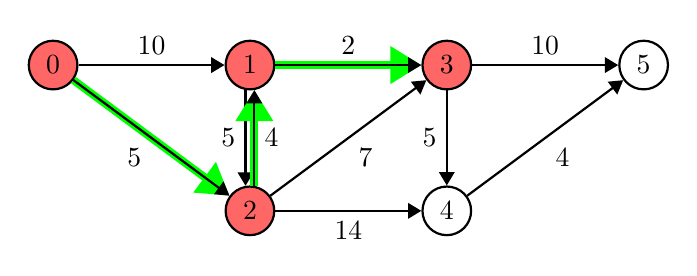
\begin{tikzpicture}[>= Triangle, node distance = 1.5 cm and 2.5cm,on grid, thick,state/.style ={circle,draw,black,text=black}]
%\node[state, fill=red!60] (0) {0};
\node[state, fill=red!60] (0) {0};
\node[state] (1) [right =of 0, fill=red!60] {1};
\node[state] (3) [right =of 1, fill=red!60] {3};
\node[state] (5) [right =of 3] {5};
\node[state] (2) [below =of 1, yshift=-10, fill=red!60] {2};
\node[state] (4) [below =of 3, yshift=-10] {4};
%\tikzset{every node/.style={fill=white}}
%https://www.overleaf.com/learn/latex/TikZ_package 
\path[->] 
		(0) edge[auto=left] node {10}				(1)
		%(0) edge[auto=right, green] 				(2)
		(0) edge[auto=right, green, line width=1mm] 	(2)
		(0) edge[auto=right] node {5}				(2)
		%(1.260) edge[auto=right, lightgray, line width=1mm]		(2.100)
		(1.260) edge[auto=right] node {5}		(2.100)
		%(1) edge[auto=left, lightgray, line width=1mm]				(3)
		(1) edge[auto=left, green, line width=1mm]				(3)
		(1) edge[auto=left] node {2}				(3)
		%(2.80) edge[auto=right, lightgray, line width=1mm]		(1.280)
		(2.80) edge[auto=right, green, line width=1mm]		(1.280)
		(2.80) edge[auto=right] node {4}		(1.280) 
		%(2) edge[auto=right, lightgray, line width=1mm]				(3)
		(2) edge[auto=right] node {7}				(3)
		%(2) edge[auto=right, lightgray, line width=1mm]			(4)
		(2) edge[auto=right] node {14}			(4)
		%(3) edge[auto=right, lightgray, line width=1mm]				(4)
		(3) edge[auto=right] node {5}				(4)
		%(3) edge[auto=left, lightgray, line width=1mm]				(5)
		(3) edge[auto=left] node {10}				(5)
		(4) edge[auto=right] node {4}				(5)
		%(c) edge [bend right=35]	(0)
		;
\end{tikzpicture}
\end{center}
\end{figure}

% https://www.khoury.northeastern.edu/home/jullman/cs3000f18/hw6.tex
% https://www.khoury.northeastern.edu/home/jullman/cs3000f18/schedule.html

%\begin{center}
D:
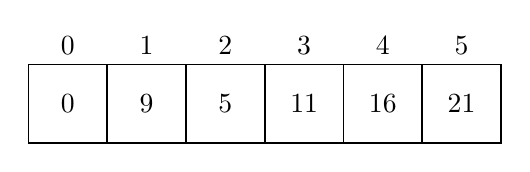
\begin{tikzpicture}[
  node distance = 0mm,
    start chain = going right,
     box/.style = {draw, semithick, minimum size=1.0cm, 
                   outer sep = 0mm, on chain}
                   ]
\foreach \i [count=\j from 0] in {0, 9, 5, 11, 16, 21}
    \node[box,label=above:\j] {\i};
\end{tikzpicture}
%\end{center}
% https://tex.stackexchange.com/questions/343409/add-text-under-tikz-rectangle


%Prioriteettijono
\begin{figure}[ht!]
\begin{center}
\begin{tikzpicture}[>= Triangle, node distance = 1.0 cm and 2.0cm,on grid, thick,state/.style ={circle,draw,black,text=black}]
%\node[state, label=right: $\infty$] (3) at (-1,2) {3};
%\node[state, label=right: 12] (3) at (-1,1) {3};
%\node[state, label=right: 11] (3) at (0,-0.5) {3};
%\node[state, label=right: $\infty$] (5) at (1,2) {5};
\node[state, label=right: 21] (5) at (0,-0.5) {5};
%\node[state, label=right: 10] (1) at (-1,1) {1};
%\node[state, label=right: 9] (1) at (0,-0.5) {1};
%\node[state, label=right: 19] (4) at (1,1) {4};
%\node[state, label=right: 16] (4) at (0,-0.5) {4};
%\node[state, label=right: 5] (2) at (0,-0.5) {2};
\node at (-2.5,0.5) {Q:};
%\tikzset{every node/.style={fill=white}}
% tikzpgfmanual.pdf p.17 
\draw[thick]
(-0.5,-2) -- (-0.5,-1) -- (-3,2.5);
\draw[thick]
(0.6,-2) -- (0.6,-1) -- (3.1,2.5);
\end{tikzpicture}
\end{center}
\end{figure}
% https://www.khoury.northeastern.edu/home/jullman/cs3000f18/hw6.tex
% https://www.khoury.northeastern.edu/home/jullman/cs3000f18/schedule.html

D = array of distances, Q = adjustable priority queue





\input{Dijkstra_2_3_step29}
\input{Dijkstra_2_3_step30}
\input{Dijkstra_2_3_step31}
\input{Dijkstra_2_3_step32}
\input{Dijkstra_2_3_step33}
\input{Dijkstra_2_3_step34}
\input{Dijkstra_2_3_step35}
\input{Dijkstra_2_3_step35}


\end{document}
